% vim: set spell spelllang=en tw=100 et sw=4 sts=4 foldmethod=marker foldmarker={{{,}}} :

\documentclass{beamer}

\usepackage{etex}
\usepackage{tikz}
\usepackage{xcolor}
\usepackage{complexity}
\usepackage{hyperref}
\usepackage{microtype}
\usepackage{amsmath}                   % \operatorname
\usepackage{amsfonts}                  % \mathcal
\usepackage{amssymb}                   % \nexists
\usepackage{gnuplot-lua-tikz}          % graphs
\usepackage[vlined]{algorithm2e} % algorithms
\usepackage{centernot}
\usepackage{mathtools}
\usepackage{listings}
\usepackage{chemfig}
\usepackage[normalem]{ulem}

\usetikzlibrary{shapes, arrows, shadows, calc, positioning, fit}
\usetikzlibrary{decorations.pathreplacing, decorations.pathmorphing, shapes.misc}
\usetikzlibrary{tikzmark}

\definecolor{uofguniversityblue}{rgb}{0, 0.219608, 0.396078}

\definecolor{uofgheather}{rgb}{0.356863, 0.32549, 0.490196}
\definecolor{uofgaquamarine}{rgb}{0.603922, 0.72549, 0.678431}
\definecolor{uofgslate}{rgb}{0.309804, 0.34902, 0.380392}
\definecolor{uofgrose}{rgb}{0.823529, 0.470588, 0.709804}
\definecolor{uofgmocha}{rgb}{0.709804, 0.564706, 0.47451}
\definecolor{uofgsandstone}{rgb}{0.321569, 0.278431, 0.231373}
\definecolor{uofgforest}{rgb}{0, 0.2, 0.129412}
\definecolor{uofglawn}{rgb}{0.517647, 0.741176, 0}
\definecolor{uofgcobalt}{rgb}{0, 0.615686, 0.92549}
\definecolor{uofgturquoise}{rgb}{0, 0.709804, 0.819608}
\definecolor{uofgsunshine}{rgb}{1.0, 0.862745, 0.211765}
\definecolor{uofgpumpkin}{rgb}{1.0, 0.72549, 0.282353}
\definecolor{uofgthistle}{rgb}{0.584314, 0.070588, 0.447059}
\definecolor{uofgrust}{rgb}{0.603922, 0.227451, 0.023529}
\definecolor{uofgburgundy}{rgb}{0.490196, 0.133333, 0.223529}
\definecolor{uofgpillarbox}{rgb}{0.701961, 0.047059, 0}
\definecolor{uofglavendar}{rgb}{0.356863, 0.301961, 0.580392}

\tikzset{vertex/.style={draw, circle, inner sep=0pt, minimum size=0.5cm, font=\small\bfseries}}
\tikzset{notvertex/.style={vertex, color=white, text=black}}
\tikzset{plainvertex/.style={vertex}}
\tikzset{vertexc1/.style={vertex, fill=uofgcobalt}}
\tikzset{vertexc2/.style={vertex, fill=uofglawn}}
\tikzset{vertexc3/.style={vertex, fill=uofgpumpkin}}
\tikzset{vertexc4/.style={vertex, fill=uofgheather}}
\tikzset{edge/.style={color=black!50!white}}
\tikzset{bedge/.style={ultra thick}}
\tikzset{edged/.style={color=screengrey, dashed}}
\tikzset{edgel3/.style={color=uofgthistle, ultra thick}}

\newcommand*\circled[1]{\tikz[baseline=(char.base)]{
            \node[shape=circle,draw,inner sep=0pt] (char) {#1};}}

% {{{ theme things
\useoutertheme[footline=authortitle]{miniframes}
\useinnertheme{rectangles}

\setbeamerfont{block title}{size={}}
\setbeamerfont{title}{size=\large,series=\bfseries}
\setbeamerfont{section title}{size=\large,series=\mdseries}
\setbeamerfont{author}{size=\normalsize,series=\mdseries}
\setbeamercolor*{structure}{fg=uofguniversityblue}
\setbeamercolor*{palette primary}{use=structure,fg=black,bg=white}
\setbeamercolor*{palette secondary}{use=structure,fg=white,bg=uofgcobalt}
\setbeamercolor*{palette tertiary}{use=structure,fg=white,bg=uofguniversityblue}
\setbeamercolor*{palette quaternary}{fg=white,bg=black}

\setbeamercolor*{titlelike}{parent=palette primary}

\beamertemplatenavigationsymbolsempty

\setbeamertemplate{title page}
{
    \begin{tikzpicture}[remember picture, overlay]
        \node at (current page.north west) {
            \begin{tikzpicture}[remember picture, overlay]
                \fill [fill=uofguniversityblue, anchor=north west] (0, 0) rectangle (\paperwidth, -2.6cm);
            \end{tikzpicture}
        };

        \node (logo) [anchor=north east, shift={(-0.6cm,-0.6cm)}] at (current page.north east) {
            \includegraphics*[keepaspectratio=true,scale=0.7]{UoG_keyline.pdf}
        };

        \node [anchor=west, xshift=0.2cm] at (current page.west |- logo.west) {
            \begin{minipage}{0.65\paperwidth}\raggedright
                {\usebeamerfont{title}\usebeamercolor[white]{}\inserttitle}\\[0.1cm]
                {\usebeamerfont{author}\usebeamercolor[white]{}\insertauthor}
            \end{minipage}
        };
    \end{tikzpicture}
}

\setbeamertemplate{section page}
{
    \begin{centering}
        \begin{beamercolorbox}[sep=12pt,center]{part title}
            \usebeamerfont{section title}\insertsection\par
        \end{beamercolorbox}
    \end{centering}
}

\newcommand{\frameofframes}{/}
\newcommand{\setframeofframes}[1]{\renewcommand{\frameofframes}{#1}}

\makeatletter
\setbeamertemplate{footline}
{%
    \begin{beamercolorbox}[colsep=1.5pt]{upper separation line foot}
    \end{beamercolorbox}
    \begin{beamercolorbox}[ht=2.5ex,dp=1.125ex,%
        leftskip=.3cm,rightskip=.3cm plus1fil]{author in head/foot}%
        \leavevmode{\usebeamerfont{author in head/foot}\insertshortauthor}%
        \hfill%
        {\usebeamerfont{institute in head/foot}\usebeamercolor[fg]{institute in head/foot}\insertshortinstitute}%
    \end{beamercolorbox}%
    \begin{beamercolorbox}[ht=2.5ex,dp=1.125ex,%
        leftskip=.3cm,rightskip=.3cm plus1fil]{title in head/foot}%
        {\usebeamerfont{title in head/foot}\insertshorttitle}%
        \hfill%
        {\usebeamerfont{frame number}\usebeamercolor[fg]{frame number}\insertframenumber~\frameofframes~\inserttotalframenumber}
    \end{beamercolorbox}%
    \begin{beamercolorbox}[colsep=1.5pt]{lower separation line foot}
    \end{beamercolorbox}
}

% }}}

\title[Solving Hard Subgraph Problems in Parallel]{Solving Hard Subgraph Problems \\ in Parallel}
\author[Ciaran McCreesh and Patrick Prosser]{\textbf{Ciaran McCreesh} and Patrick Prosser}

\begin{document}

{
    \usebackgroundtemplate{
        \tikz[overlay, remember picture]
        \node[at=(current page.south), anchor=south, inner sep=0pt]{\includegraphics*[keepaspectratio=true, width=\paperwidth]{background.jpg}};
    }
    \begin{frame}[plain,noframenumbering]
        \titlepage
    \end{frame}
}

\begin{frame}{Subgraph Isomorphism}
    \begin{center}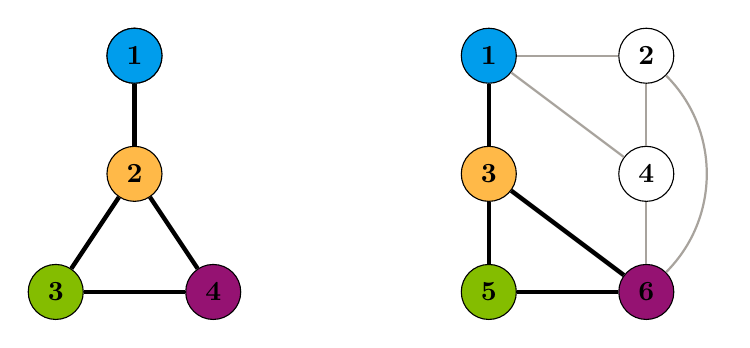
\begin{tikzpicture}
        \node [draw, circle, fill=white, inner sep=4pt, font=\bfseries] (Na) at (1,  0) {1};
            \node [draw, circle, fill=uofgcobalt, inner sep=4pt, font=\bfseries] (Na) at (1,  0) {1};
            \node [draw, circle, fill=uofgpumpkin, inner sep=4pt, font=\bfseries] (Nb) at (1, -1.5) {2};
            \node [draw, circle, fill=uofglawn, inner sep=4pt, font=\bfseries] (Nc) at (0, -3) {3};
            \node [draw, circle, fill=uofgthistle, inner sep=4pt, font=\bfseries] (Nd) at (2, -3) {4};

            \draw [ultra thick] (Na) -- (Nb);
            \draw [ultra thick] (Nb) -- (Nc);
            \draw [ultra thick] (Nc) -- (Nd);
            \draw [ultra thick] (Nb) -- (Nd);

            \node [draw, circle, fill=uofgcobalt, inner sep=4pt, font=\bfseries] (N1) at (5.5,  0) {1};
            \node [draw, circle, fill=white, inner sep=4pt, font=\bfseries] (N2) at (7.5,  0) {2};
            \node [draw, circle, fill=uofgpumpkin, inner sep=4pt, font=\bfseries] (N3) at (5.5, -1.5) {3};
            \node [draw, circle, fill=white, inner sep=4pt, font=\bfseries] (N4) at (7.5, -1.5) {4};
            \node [draw, circle, fill=uofglawn, inner sep=4pt, font=\bfseries] (N5) at (5.5, -3) {5};
            \node [draw, circle, fill=uofgthistle, inner sep=4pt, font=\bfseries] (N6) at (7.5, -3) {6};

            \draw [thick, color=uofgsandstone!50] (N1) -- (N2);
            \draw [ultra thick] (N1) -- (N3);
            \draw [thick, color=uofgsandstone!50] (N1) -- (N4);
            \draw [thick, color=uofgsandstone!50] (N2) -- (N4);
            \draw [ultra thick] (N3) -- (N5);
            \draw [ultra thick] (N3) -- (N6);
            \draw [thick, color=uofgsandstone!50] (N4) -- (N6);
            \draw [ultra thick] (N5) -- (N6);
            \draw [thick, color=uofgsandstone!50] (N2) to [in=45, out=315] (N6);
    \end{tikzpicture}\end{center}

\end{frame}

\begin{frame}{The Maximum Clique Problem}
    \begin{center}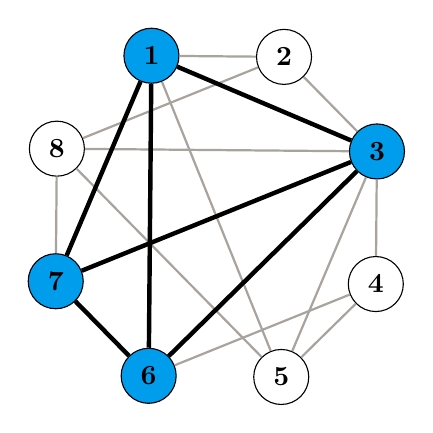
\begin{tikzpicture}
        \newcount \c
        \foreach \n in {1, ..., 8}{
            \c=\n \advance\c by -1 \multiply\c by -360 \divide\c by 8 \advance\c by 112.5
            \ifthenelse{\n = 1 \OR \n = 3 \OR \n = 6 \OR \n = 7}{
                \node[draw, circle, fill=uofgcobalt, inner sep=4pt, font=\bfseries] (N\n) at (\the\c:2.2) {\n};
            }{
                \node[draw, circle, fill=white, inner sep=4pt, font=\bfseries] (N\n) at (\the\c:2.2) {\n};
            }
        }

        \draw [thick, color=uofgsandstone!50] (N1) -- (N2);
        \draw [thick, color=uofgsandstone!50] (N1) -- (N5);
        \draw [thick, color=uofgsandstone!50] (N2) -- (N3);
        \draw [thick, color=uofgsandstone!50] (N2) -- (N8);
        \draw [thick, color=uofgsandstone!50] (N3) -- (N4);
        \draw [thick, color=uofgsandstone!50] (N3) -- (N5);
        \draw [thick, color=uofgsandstone!50] (N3) -- (N8);
        \draw [thick, color=uofgsandstone!50] (N4) -- (N5);
        \draw [thick, color=uofgsandstone!50] (N4) -- (N6);
        \draw [thick, color=uofgsandstone!50] (N5) -- (N8);
        \draw [thick, color=uofgsandstone!50] (N7) -- (N8);

        \draw [ultra thick] (N1) -- (N3);
        \draw [ultra thick] (N1) -- (N6);
        \draw [ultra thick] (N1) -- (N7);
        \draw [ultra thick] (N3) -- (N6);
        \draw [ultra thick] (N3) -- (N7);
        \draw [ultra thick] (N6) -- (N7);
    \end{tikzpicture}\end{center}

\end{frame}

\begin{frame}{Maximum Common Subgraph}
    \begin{center}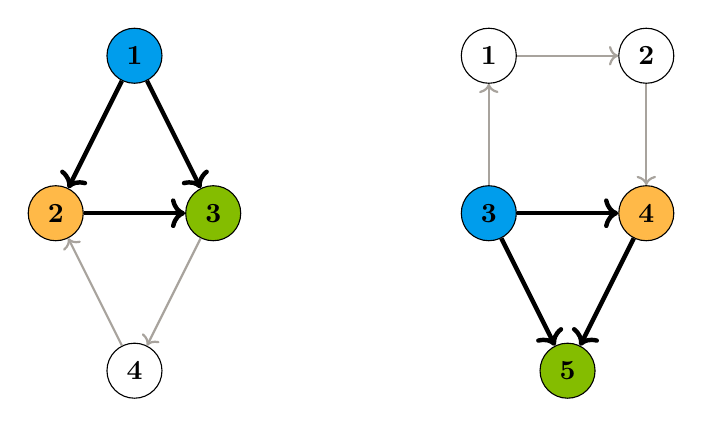
\begin{tikzpicture}%{{{
        \node[draw, circle, fill=uofgcobalt, inner sep=4pt, font=\bfseries] (Ma) at (1, -7.5) {1};
        \node[draw, circle, fill=uofgpumpkin, inner sep=4pt, font=\bfseries] (Mb) at (0, -9.5) {2};
        \node[draw, circle, fill=uofglawn, inner sep=4pt, font=\bfseries] (Mc) at (2, -9.5) {3};
        \node[draw, circle, fill=white, inner sep=4pt, font=\bfseries] (Md) at (1, -11.5) {4};

        \node[draw, circle, fill=white, inner sep=4pt, font=\bfseries] (M1) at (5.5, -7.5) {1};
        \node[draw, circle, fill=white, inner sep=4pt, font=\bfseries] (M2) at (7.5, -7.5) {2};
        \node[draw, circle, fill=uofgcobalt, inner sep=4pt, font=\bfseries] (M3) at (5.5, -9.5) {3};
        \node[draw, circle, fill=uofgpumpkin, inner sep=4pt, font=\bfseries] (M4) at (7.5, -9.5) {4};
        \node[draw, circle, fill=uofglawn, inner sep=4pt, font=\bfseries] (M5) at (6.5, -11.5) {5};

        \draw [->, thick, color=uofgsandstone!50] (Mc) -> (Md);
        \draw [->, thick, color=uofgsandstone!50] (Md) -- (Mb);
        \draw [->, ultra thick] (Ma) -> (Mb);
        \draw [->, ultra thick] (Mb) -> (Mc);
        \draw [->, ultra thick] (Ma) -> (Mc);

        \draw [->, thick, color=uofgsandstone!50] (M1) -> (M2);
        \draw [->, thick, color=uofgsandstone!50] (M2) -> (M4);
        \draw [->, thick, color=uofgsandstone!50] (M3) -> (M1);
        \draw [->, ultra thick] (M3) -> (M4);
        \draw [->, ultra thick] (M3) -> (M5);
        \draw [->, ultra thick] (M4) -> (M5);
    \end{tikzpicture}\end{center}
\end{frame}

\begin{frame}{Thread-Parallel Tree Search}

    \only<1-3> {
        \centering
        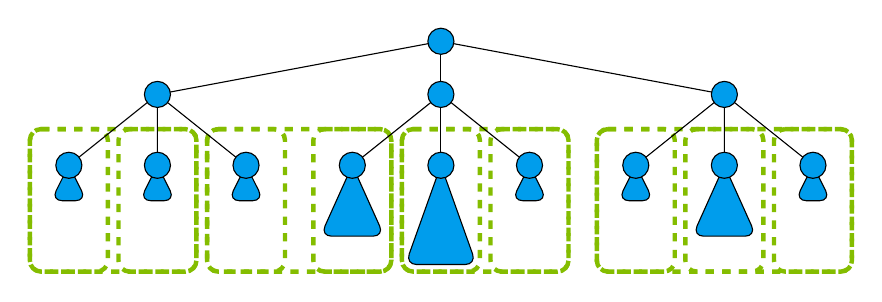
\begin{tikzpicture}[scale=0.9]%{{{
            \coordinate (R);

            \coordinate (N) at (R);

            \coordinate (N1) at ($(N) + (-4, -0.75)$);
            \coordinate (N2) at ($(N) + ( 0, -0.75)$);
            \coordinate (N3) at ($(N) + ( 4, -0.75)$);

            \foreach \na in {1, ..., 3}{
                \coordinate (N\na 1) at ($(N\na) + (-1.25, -1)$);
                \coordinate (N\na 2) at ($(N\na) + ( 0,    -1)$);
                \coordinate (N\na 3) at ($(N\na) + ( 1.25, -1)$);

                \foreach \nb in {1, ..., 3}{
                    \coordinate (N\na\nb t1) at ($(N\na\nb) + (-0.45, -1)$);
                    \coordinate (N\na\nb t2) at ($(N\na\nb) + ( 0.45, -1)$);

                    \coordinate (N\na\nb s1) at ($(N\na\nb) + (-0.25, -0.5)$);
                    \coordinate (N\na\nb s2) at ($(N\na\nb) + ( 0.25, -0.5)$);

                    \coordinate (N\na\nb h1) at ($(N\na\nb) + (-0.5, -1.4)$);
                    \coordinate (N\na\nb h2) at ($(N\na\nb) + ( 0.5, -1.4)$);
                }
            }

            \tikzstyle{i} = [draw, rounded corners, dashed, color=white, ultra thick];
            \draw <1> [i] ($(N11) + (-0.55, 0.51)$) -- ($(N12) + (0.55, 0.51)$) -- ($(N12) + (0.55, -1.5)$) -- ($(N11) + (-0.55, -1.5)$) -- cycle;
            \draw <1> [i] ($(N13) + (-0.55, 0.51)$) -- ($(N21) + (0.55, 0.51)$) -- ($(N21) + (0.55, -1.5)$) -- ($(N13) + (-0.55, -1.5)$) -- cycle;
            \draw <1> [i] ($(N22) + (-0.55, 0.51)$) -- ($(N23) + (0.55, 0.51)$) -- ($(N23) + (0.55, -1.5)$) -- ($(N22) + (-0.55, -1.5)$) -- cycle;
            \draw <1> [i] ($(N31) + (-0.55, 0.51)$) -- ($(N33) + (0.55, 0.51)$) -- ($(N33) + (0.55, -1.5)$) -- ($(N31) + (-0.55, -1.5)$) -- cycle;

            \tikzstyle{p} = [draw, rounded corners, dashed, color=uofglawn, ultra thick];
            \draw <2> [p] ($(N11) + (-0.55, 0.51)$) -- ($(N12) + (0.55, 0.51)$) -- ($(N12) + (0.55, -1.5)$) -- ($(N11) + (-0.55, -1.5)$) -- cycle;
            \draw <2> [p] ($(N13) + (-0.55, 0.51)$) -- ($(N21) + (0.55, 0.51)$) -- ($(N21) + (0.55, -1.5)$) -- ($(N13) + (-0.55, -1.5)$) -- cycle;
            \draw <2> [p] ($(N22) + (-0.55, 0.51)$) -- ($(N23) + (0.55, 0.51)$) -- ($(N23) + (0.55, -1.5)$) -- ($(N22) + (-0.55, -1.5)$) -- cycle;
            \draw <2> [p] ($(N31) + (-0.55, 0.51)$) -- ($(N33) + (0.55, 0.51)$) -- ($(N33) + (0.55, -1.5)$) -- ($(N31) + (-0.55, -1.5)$) -- cycle;

            \foreach \na in {1, ..., 3}{
                \foreach \nb in {1, ..., 3}{
                    \draw <3> [p] ($(N\na\nb) + (-0.55, 0.51)$) -- ($(N\na\nb) + (0.55, 0.51)$) --
                    ($(N\na\nb) + (0.55, -1.5)$) -- ($(N\na\nb) + (-0.55, -1.5)$) -- cycle;
                }
            }

            \foreach \na in {1, ..., 3}{
                \draw (N) -- (N\na);
                \foreach \nb in {1, ..., 3}{
                    \draw (N\na) -- (N\na\nb);
                }
            }

            \tikzstyle{t} = [draw, fill, fill=uofgcobalt, rounded corners];

            \draw [t] (N11) -- (N11s1) -- (N11s2) -- cycle;
            \draw [t] (N12) -- (N12s1) -- (N12s2) -- cycle;
            \draw [t] (N13) -- (N13s1) -- (N13s2) -- cycle;

            \draw [t] (N21) -- (N21t1) -- (N21t2) -- cycle;
            \draw [t] (N22) -- (N22h1) -- (N22h2) -- cycle;
            \draw [t] (N23) -- (N23s1) -- (N23s2) -- cycle;

            \draw [t] (N31) -- (N31s1) -- (N31s2) -- cycle;
            \draw [t] (N32) -- (N32t1) -- (N32t2) -- cycle;
            \draw [t] (N33) -- (N33s1) -- (N33s2) -- cycle;

            \tikzstyle{c} = [draw, circle, fill, fill=uofgcobalt];
            \node [c] at (N) { };

            \foreach \na in {1, ..., 3}{
                \node [c] at (N\na) { };

                \foreach \nb in {1, ..., 3}{
                    \node [c] at (N\na\nb) { };
                }
            }
        \end{tikzpicture}%}}}
    }

\end{frame}

\begin{frame}{Parallel Search Order Matters}
    \only<1> {
        \begin{center}\input{gen-graph-speedup.tex}\end{center}
    }
    \only<2> {
        \begin{center}\input{gen-graph-speedup-2.tex}\end{center}
    }
\end{frame}

\begin{frame}{Safety and Reproducibility in Parallel Search}

    \begin{itemize}
        \item My ``wish list'':
            \begin{enumerate}
                \item Parallel search should \textbf{not be substantially
                    slower} than sequential search.
                \item Adding more processors should \textbf{not make things
                    substantially worse}.
                \item Running the same program twice on the same hardware
                    should give \textbf{similar runtimes}.
            \end{enumerate}
        \item This is surprisingly tricky.
        \item On top of all that, we want to \textbf{prioritise work stealing}
            from where we're most likely to be wrong.
    \end{itemize}
\end{frame}

\begin{frame}{Graph Algorithms and Optimisation}

    \begin{itemize}
        \item There are a lot of real-world optimisation problems involving \textbf{a
            graph problem} (subgraph isomorphism, subgraph covering, finding
            sequences of related subgraphs, clique finding, graph colouring,
            \ldots), plus some \textbf{other constraints}.

        \item Can we make these problems easier to specify in a \textbf{high-level constraint
            modelling language} like MiniZinc?

        \item There is a continuum of what we could do with these models:

            \begin{itemize}

                \item Compile to CP, MIP or SAT (but these models tend to be large, and lose
                    structural and heuristic information).
                \item A hybrid, multi-solver approach, ``graph morphisms modulo theories'' style
                    (but we need better theories).
                \item Compile to subgraph isomorphism (but even simple arithmetic constraints become
                    disgusting under reduction).

            \end{itemize}
    \end{itemize}
\end{frame}

\begin{frame}[plain,noframenumbering]
    \begin{center}
        \vspace*{4em}
        \url{http://www.dcs.gla.ac.uk/~ciaran} \\
        \vspace{1em}
        \href{mailto:c.mccreesh.1@research.gla.ac.uk}{\nolinkurl{c.mccreesh.1@research.gla.ac.uk}} \\
    \end{center}

    \begin{tikzpicture}[remember picture, overlay]
        \node at (current page.north west) {
            \begin{tikzpicture}[remember picture, overlay]
                \fill [fill=uofguniversityblue, anchor=north west] (0, 0) rectangle (\paperwidth, -2.6cm);
            \end{tikzpicture}
        };

        \node (logo) [anchor=north east, shift={(-0.6cm,-0.6cm)}] at (current page.north east) {
            \includegraphics*[keepaspectratio=true,scale=0.7]{UoG_keyline.pdf}
        };
    \end{tikzpicture}
\end{frame}

\end{document}

